\chapter{Notes}
\section{extra refs}


\subsection{Introduction synapses}
\textcolor{red}{review}
@article{humeau2019next,
  title={The next generation of approaches to investigate the link between synaptic plasticity and learning},
  author={Humeau, Yann and Choquet, Daniel},
  journal={Nature neuroscience},
  volume={22},
  number={10},
  pages={1536--1543},
  year={2019},
  publisher={Nature Publishing Group}
}

\subsection{centrality measures}
@article{valente2008correlated,
  title={How correlated are network centrality measures?},
  author={Valente, Thomas W and Coronges, Kathryn and Lakon, Cynthia and Costenbader, Elizabeth},
  journal={Connections (Toronto, Ont.)},
  volume={28},
  number={1},
  pages={16},
  year={2008},
  publisher={NIH Public Access}
}

@inproceedings{koschutzki2004comparison,
  title={Comparison of centralities for biological networks},
  author={Kosch{\"u}tzki, Dirk and Schreiber, Falk},
  booktitle={German Conference on Bioinformatics 2004, GCB 2004},
  year={2004},
  organization={Gesellschaft f{\"u}r Informatik eV}
}

@article{jalili2016evolution,
  title={Evolution of centrality measurements for the detection of essential proteins in biological networks},
  author={Jalili, Mahdi and Salehzadeh-Yazdi, Ali and Gupta, Shailendra and Wolkenhauer, Olaf and Yaghmaie, Marjan and Resendis-Antonio, Osbaldo and Alimoghaddam, Kamran},
  journal={Frontiers in Physiology},
  volume={7},
  pages={375},
  year={2016},
  publisher={Frontiers}
}

\subsection{communities}
\textcolor{red}{Over 1000 citations}
@article{porter2009communities,
  title={Communities in networks},
  author={Porter, Mason A and Onnela, Jukka-Pekka and Mucha, Peter J},
  journal={Notices of the AMS},
  volume={56},
  number={9},
  pages={1082--1097},
  year={2009}
}

\textcolor{red}{cited by 853}
@article{good2010performance,
  title={Performance of modularity maximization in practical contexts},
  author={Good, Benjamin H and De Montjoye, Yves-Alexandre and Clauset, Aaron},
  journal={Physical Review E},
  volume={81},
  number={4},
  pages={046106},
  year={2010},
  publisher={APS}
}

\textcolor{red}{citations 97}
@article{lewis2010function,
  title={The function of communities in protein interaction networks at multiple scales},
  author={Lewis, Anna CF and Jones, Nick S and Porter, Mason A and Deane, Charlotte M},
  journal={BMC systems biology},
  volume={4},
  number={1},
  pages={100},
  year={2010},
  publisher={Springer}
}

\textcolor{red}{cited by 8635}
@article{fortunato2010community,
  title={Community detection in graphs},
  author={Fortunato, Santo},
  journal={Physics reports},
  volume={486},
  number={3-5},
  pages={75--174},
  year={2010},
  publisher={Elsevier}
}

\textcolor{red}{cited by 457}
@article{lancichinetti2012consensus,
  title={Consensus clustering in complex networks},
  author={Lancichinetti, Andrea and Fortunato, Santo},
  journal={Scientific reports},
  volume={2},
  pages={336},
  year={2012},
  publisher={Nature Publishing Group}
}

\textcolor{red}{cited by 877}
@article{lancichinetti2011finding,
  title={Finding statistically significant communities in networks},
  author={Lancichinetti, Andrea and Radicchi, Filippo and Ramasco, Jos{\'e} J and Fortunato, Santo},
  journal={PloS one},
  volume={6},
  number={4},
  year={2011},
  publisher={Public Library of Science}
}

\subsection{multilayer networks}@article{humeau2019next,
  title={The next generation of approaches to investigate the link between synaptic plasticity and learning},
  author={Humeau, Yann and Choquet, Daniel},
  journal={Nature neuroscience},
  volume={22},
  number={10},
  pages={1536--1543},
  year={2019},
  publisher={Nature Publishing Group}
}

\textcolor{red}{cited by 1936}
@article{kivela2014multilayer,
  title={Multilayer networks},
  author={Kivel{\"a}, Mikko and Arenas, Alex and Barthelemy, Marc and Gleeson, James P and Moreno, Yamir and Porter, Mason A},
  journal={Journal of complex networks},
  volume={2},
  number={3},
  pages={203--271},
  year={2014},
  publisher={Oxford University Press}
}

\textcolor{red}{over 100 pages, cited by 1878}
@article{boccaletti2014structure,
  title={The structure and dynamics of multilayer networks},
  author={Boccaletti, Stefano and Bianconi, Ginestra and Criado, Regino and Del Genio, Charo I and G{\'o}mez-Gardenes, Jes{\'u}s and Romance, Miguel and Sendina-Nadal, Irene and Wang, Zhen and Zanin, Massimiliano},
  journal={Physics Reports},
  volume={544},
  number={1},
  pages={1--122},
  year={2014},
  publisher={Elsevier}
}



\subsection{general notes}
Wagner and Fell small world

\subsection{extra results}
Enrichment of new graph components


 MEAN SAMPLE\ SIZE = 250000
 TOTAL GENES = 18673
 CONDITIONED INTERNAL = genesize, log genesize, genedensity, log genedensity, inverse mac, log inverse mac
SET           NGENES       BETA   BETA STD         SE            P
new in graph    1397     0.0553     0.0145     0.0293     0.029806
new graph       4414      0.101     0.0427     0.0186   3.1989e-08
PSD             3414      0.113     0.0436     0.0201   1.0565e-08



\section{Readme from Sniekers}
\label{sec:notes readme from sniekers}

Uses NCBI 37.3 in MAGMA

     Association results of the meta-analysis for intelligence based on 78,308 individuals in 13 cohorts. 
     Version date: 10-07-2017

  Columns:
Chromosome: chromosome number
position: base pair position of the SNP on the chromosome (reported on GRCh37)
rsid: SNP rs number
ref: effect allele
alt: non-effect allele
N: sample size
MAF: minor allele frequency in UK Biobank
Beta: effect size of the effect allele
SE: standard error of the effect
Zscore: Z-score computed in METAL by a weighted Z-score method
p   value: P-value computed in METAL by a weighted Z-score method
direction: direction of the effect in each of the cohorts, order: CHIC (consisting of 6 cohorts), UKB-wb, UKB-ts, ERF, GENR, HU, MCTFR, STR

Beta/SE were calculated from METAL Z-scores using the formula from Zhu et al (Nature Genetics, 2016):

Beta = Zscore / sqrt( 2 * MAF * ( 1 - MAF) * ( N + $Zscore^2$ ) )
SE = 1 / sqrt( 2 * MAF * ( 1 - MAF ) * ( N + $Zscore^2$ ) )

\section{Useful papers for methods}

MDD for quoting MAGMA \url{https://www.nature.com/articles/s41467-018-03819-3}

\section{Community detection}

Communities allow the network to be broken up into smaller components which can be analysed in turn and which may represent functional units.


\section{Modularity}

for an adjacency matrix $A_{ij}$ we want to know how many edges pass between similar nodes that share a property be it an ontology term or a community membership.

Total number of edges is between nodes of same group is:

\begin{equation}
\label{eq:notes_modularity_totaledges}
    \frac{1}{2} \sum_{i,j} A_{i,j}\delta_{g_i g_j}
\end{equation}

The expected number of edges between all nodes of the same type is 

\begin{equation}
    \frac{1}{2}\sum_{i,j} \frac{k_i k_j}{2m}\delta_{g_i g_j}
\end{equation}

The modularity Q is 

\begin{equation}
    Q=\frac{1}{2m}\sum_{i,j}\textcolor{red}{(A_{i,j}-\frac{k_i k_j}{2m}}) \delta{g_i g_j}
\end{equation}

The red term is:

\begin{equation}
    B_{ij} = \sum_{i,j} A_{i,j} - \frac{k_i k_j}{2m}
\end{equation}

$\mathbf{B}$ is the modularity matrix which is n by n having elements $B_{i,j}$



\section{Centrality measures}
Betweeness, degree and closeness were described by Freeman, eigenvector centrality by Bonich \cite{valente2008correlated}

Boland degree closeness and flow centrality correlated but betweenness not

The correlation of symmetrised centrality measures are shown in table~\ref{tab:Correlation of centrality valente et al}. This study addressed 58 sociometric networks. The networks were directed and in order to calculated eigenvector centrality the networks were ``symmetrised" as described by the authors or made undirected. Degree had the strongest overall correlation 0.7 followed by eigenvector centrality 0.67.

\section{Top GO}
Using Fisher's exact test in topGO.
\subsection{Spectral clustering}

Results for gene set enrichment using topgo most significant group for ontology term biological process (see table~\ref{tab:Top term biological process spectral clustering background PSP}. 10969 terms are present in the BP terms list so I have included an adjusted alpha of 0.05/10969 = $4.56 \times 10^{-6}$ however the terms in GO are not independent and classical correction for multiple comparisons may be complicated. 

Results for molecular function against background of PSP are shown in table~\ref{tab:Top term molecular function spectral clustering background PSP}. There are 2473 terms in the topGO Molecular Function list $\alpha=$ 0.05/2473 = $2.02 \times 10^{-5}$

Results for cellular component against background of PSP are shown in table~\ref{tab:Top term CC background spectral clustering PSP}. There are 1499 terms in the topGO Cellular component list $\alpha=$0.05/1499 = $3.36 \times 10^{-5}$.


\subsection{Permutation of labels}
Simulated 
BP only one significant term at $3.00 \times 10^{-5}$
Summary
   Min.  1st Qu.   Median     Mean  3rd Qu.     Max. 
0.000030 0.000280 0.000940 0.001088 0.001450 0.005400 

Non simulaterd
% latex table generated in R 3.6.3 by xtable 1.8-4 package
% Sat Apr 18 17:32:34 2020
\begin{table}[ht]
\centering
\begin{tabular}{lr}
  \hline
quantile & value of p \\ 
  \hline
0\% & $1.000 \times 10^{-30}$ \\ 
  25\% & $6.250 \times 10^{-19}$ \\ 
  50\% & $1.300 \times 10^{-12}$ \\ 
  75\% & $8.250 \times 10^{-7}$ \\ 
  100\% & $3.900 \times 10^{-4}$ \\ 
   \hline
\end{tabular}
\caption{P values for different quantiles for BP} 
\label{tabP values for different quantiles for BP}
\end{table}

% latex table generated in R 3.6.3 by xtable 1.8-4 package
% Sat Apr 18 17:35:47 2020
\begin{table}[ht]
\centering
\begin{tabular}{lr}
  \hline
quantile & value of p \\ 
  \hline
0\% & $1.000 \times 10^{-30}$ \\ 
  25\% & $5.541 \times 10^{-14}$ \\ 
  50\% & $2.300 \times 10^{-7}$ \\ 
  75\% & $4.600 \times 10^{-5}$ \\ 
  100\% & $2.500 \times 10^{-3}$ \\ 
   \hline
\end{tabular}
\caption{P values for different quantiles for MF} 
\label{tabP values for different quantiles for MF}
\end{table}

% latex table generated in R 3.6.3 by xtable 1.8-4 package
% Sat Apr 18 17:39:43 2020
\begin{table}[ht]
\centering
\begin{tabular}{lr}
  \hline
quantile & value of p \\ 
  \hline
0\% & $1.000 \times 10^{-30}$ \\ 
  25\% & $1.300 \times 10^{-17}$ \\ 
  50\% & $1.100 \times 10^{-10}$ \\ 
  75\% & $1.350 \times 10^{-7}$ \\ 
  100\% & $9.700 \times 10^{-3}$ \\ 
   \hline
\end{tabular}
\caption{P values for different quantiles for CC} 
\label{tabP values for different quantiles for CC}
\end{table}
Median 1.3e-12
Mean 2.637653e-05
31 significant terms


	Paired t-test


t = 4.5857, df = 34, p-value = 5.878e-05 BP
alternative hypothesis: true difference in means is not equal to 0
95 percent confidence interval:
 0.0007240725 0.0018766167
sample estimates:
mean of the differences 
            0.001300345 

perhaps with the benchmarks in the real network there are elements with weak communtity structure ie how to evaluate the good performance of infomap especially when there is a minimum groups size of ten and it normally finds lots with one member in the group.    

Given that the singles are not assigned to groups due to size criteria it may be worth having a statistic of number of nodes in single group or even gamma for the community size distribution.

Boxplot of the difference in p values between spectral groups and random groups of same size from PSP is shown in figure~\ref{fig:topGO_permutation}
\begin{figure}
    \centering
    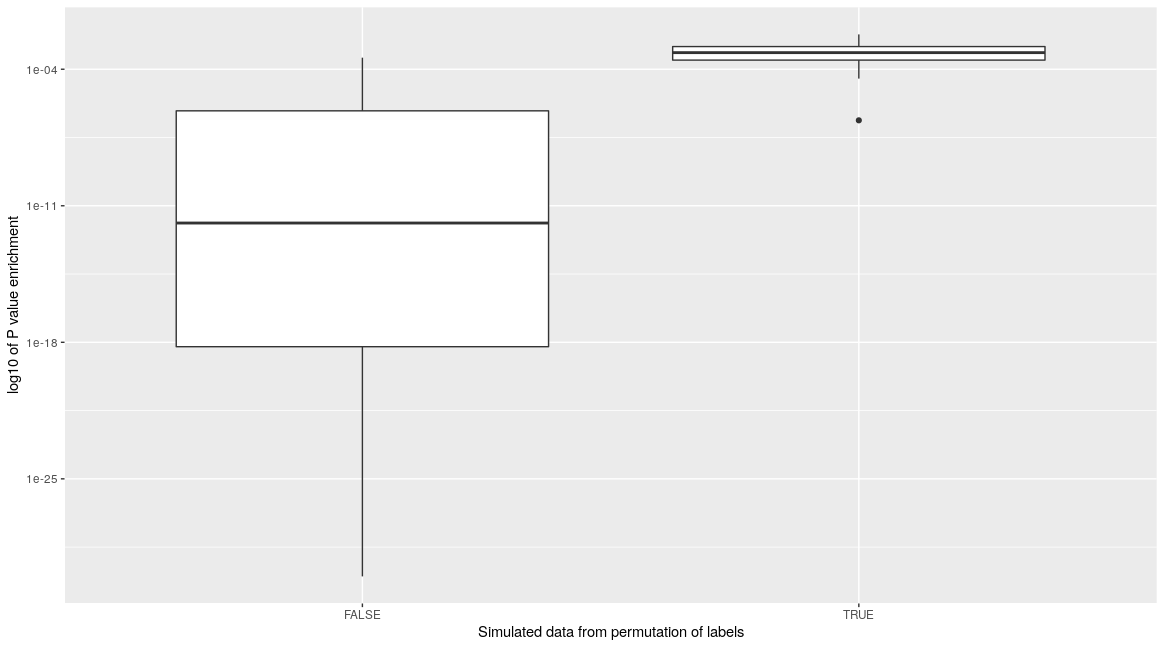
\includegraphics[width=0.9\textwidth]{images/Rplot_EnrichmentGO_permuted_labels.png}
    \caption{Enrichment p values for spectral groups Biological Process left compared with enrichment p values for groups of identical size derived from label permutation. Top p value for each group used.}
    \label{fig:topGO_permutation}
\end{figure}
% latex table generated in R 3.6.3 by xtable 1.8-4 package
% Sat Apr 11 15:28:29 2020
\begin{table}[ht]
\centering
\begin{adjustbox}{max width=\textwidth}
\begin{tabular}{lllrrrrl}
  \hline
community & GO.ID & Term & Annotated & Significant & Expected & classic & less\_than\_alpha \\ 
  \hline
1 & GO:0000226 & microtubule cytoskeleton organization & 201 & 44 & 9.64 & $3.20 \times 10^{-19}$ & TRUE \\ 
  2 & GO:0031145 & anaphase-promoting complex-dependent cat... & 34 & 30 & 1.64 & $1.00 \times 10^{-30}$ & TRUE \\ 
  3 & GO:0034762 & regulation of transmembrane transport & 203 & 10 & 2.25 & $4.60 \times 10^{-5}$ & FALSE \\ 
  4 & GO:0007031 & peroxisome organization & 36 & 13 & 0.33 & $4.30 \times 10^{-19}$ & TRUE \\ 
  5 & GO:0007186 & G protein-coupled receptor signaling pat... & 178 & 34 & 5.71 & $8.20 \times 10^{-19}$ & TRUE \\ 
  6 & GO:0097035 & regulation of membrane lipid distributio... & 9 & 5 & 0.19 & $4.50 \times 10^{-7}$ & TRUE \\ 
  7 & GO:0061640 & cytoskeleton-dependent cytokinesis & 50 & 11 & 1.84 & $1.20 \times 10^{-6}$ & TRUE \\ 
  9 & GO:0001894 & tissue homeostasis & 56 & 10 & 1.06 & $5.00 \times 10^{-8}$ & TRUE \\ 
  10 & GO:0042773 & ATP synthesis coupled electron transport & 56 & 43 & 2.57 & $1.00 \times 10^{-30}$ & TRUE \\ 
  11 & GO:0034498 & early endosome to Golgi transport & 5 & 3 & 0.08 & $3.70 \times 10^{-5}$ & FALSE \\ 
  12 & GO:0007041 & lysosomal transport & 51 & 14 & 0.50 & $3.70 \times 10^{-18}$ & TRUE \\ 
  16 & GO:0000045 & autophagosome assembly & 34 & 10 & 0.73 & $1.00 \times 10^{-9}$ & TRUE \\ 
  17 & GO:0061025 & membrane fusion & 70 & 28 & 2.92 & $9.40 \times 10^{-22}$ & TRUE \\ 
  19 & GO:0046755 & viral budding & 13 & 5 & 0.08 & $5.60 \times 10^{-9}$ & TRUE \\ 
  20 & GO:0006468 & protein phosphorylation & 535 & 65 & 23.57 & $9.70 \times 10^{-17}$ & TRUE \\ 
  22 & GO:0046328 & regulation of JNK cascade & 47 & 6 & 0.59 & $2.00 \times 10^{-5}$ & FALSE \\ 
  23 & GO:1900028 & negative regulation of ruffle assembly & 2 & 2 & 0.04 & $3.90 \times 10^{-4}$ & FALSE \\ 
  24 & GO:0006470 & protein dephosphorylation & 101 & 13 & 2.27 & $2.20 \times 10^{-7}$ & TRUE \\ 
  25 & GO:0072321 & chaperone-mediated protein transport & 7 & 3 & 0.06 & $1.60 \times 10^{-5}$ & FALSE \\ 
  26 & GO:0043408 & regulation of MAPK cascade & 172 & 33 & 6.08 & $7.40 \times 10^{-17}$ & TRUE \\ 
  28 & GO:1903361 & protein localization to basolateral plas... & 6 & 3 & 0.06 & $2.30 \times 10^{-5}$ & FALSE \\ 
  32 & GO:0051480 & regulation of cytosolic calcium ion conc... & 87 & 12 & 1.28 & $1.90 \times 10^{-9}$ & TRUE \\ 
  33 & GO:0006897 & endocytosis & 278 & 55 & 15.66 & $2.70 \times 10^{-18}$ & TRUE \\ 
  34 & GO:0007015 & actin filament organization & 172 & 60 & 10.62 & $1.00 \times 10^{-30}$ & TRUE \\ 
  43 & GO:0051276 & chromosome organization & 238 & 71 & 10.34 & $1.00 \times 10^{-30}$ & TRUE \\ 
  44 & GO:0006457 & protein folding & 102 & 25 & 3.06 & $2.60 \times 10^{-17}$ & TRUE \\ 
  45 & GO:0036503 & ERAD pathway & 27 & 13 & 0.98 & $1.30 \times 10^{-12}$ & TRUE \\ 
  46 & GO:0070202 & regulation of establishment of protein l... & 8 & 8 & 0.11 & $8.30 \times 10^{-16}$ & TRUE \\ 
  47 & GO:0035337 & fatty-acyl-CoA metabolic process & 19 & 3 & 0.15 & $3.70 \times 10^{-4}$ & FALSE \\ 
  48 & GO:0006183 & GTP biosynthetic process & 3 & 3 & 0.02 & $2.50 \times 10^{-7}$ & TRUE \\ 
  51 & GO:0006409 & tRNA export from nucleus & 12 & 9 & 0.40 & $6.70 \times 10^{-12}$ & TRUE \\ 
  53 & GO:0006413 & translational initiation & 120 & 106 & 14.17 & $1.00 \times 10^{-30}$ & TRUE \\ 
  55 & GO:0006397 & mRNA processing & 95 & 16 & 1.22 & $7.30 \times 10^{-15}$ & TRUE \\ 
  58 & GO:2001235 & positive regulation of apoptotic signali... & 53 & 6 & 0.59 & $1.90 \times 10^{-5}$ & FALSE \\ 
  62 & GO:0070125 & mitochondrial translational elongation & 32 & 15 & 0.32 & $1.00 \times 10^{-23}$ & TRUE \\ 
   \hline
\end{tabular}
\end{adjustbox}
\caption{Top term biological process Spectral clustering background PSP} 
\label{tab:Top term biological process spectral clustering background PSP}
\end{table}

% latex table generated in R 3.6.3 by xtable 1.8-4 package
% Sat Apr 11 15:39:02 2020
\begin{table}[ht]
\centering
\begin{adjustbox}{max width=\textwidth}
\begin{tabular}{lllrrrrl}
  \hline
community & GO.ID & Term & Annotated & Significant & Expected & classic & less\_than\_alpha \\ 
  \hline
1 & GO:0008017 & microtubule binding & 113 & 21 & 5.12 & $1.50 \times 10^{-8}$ & TRUE \\ 
  2 & GO:0004298 & threonine-type endopeptidase activity & 13 & 13 & 0.62 & $4.50 \times 10^{-18}$ & TRUE \\ 
  3 & GO:0008270 & zinc ion binding & 119 & 7 & 1.40 & $3.90 \times 10^{-4}$ & FALSE \\ 
  4 & GO:0031489 & myosin V binding & 14 & 4 & 0.13 & $5.90 \times 10^{-6}$ & TRUE \\ 
  5 & GO:0008066 & glutamate receptor activity & 21 & 12 & 0.66 & $1.10 \times 10^{-13}$ & TRUE \\ 
  6 & GO:0015247 & aminophospholipid transmembrane transpor... & 3 & 3 & 0.06 & $9.50 \times 10^{-6}$ & TRUE \\ 
  7 & GO:0005525 & GTP binding & 159 & 19 & 5.82 & $3.10 \times 10^{-6}$ & TRUE \\ 
  9 & GO:0005507 & copper ion binding & 12 & 4 & 0.23 & $5.30 \times 10^{-5}$ & FALSE \\ 
  10 & GO:0003954 & NADH dehydrogenase activity & 33 & 31 & 1.51 & $1.00 \times 10^{-30}$ & TRUE \\ 
  11 & GO:1990460 & leptin receptor binding & 3 & 3 & 0.05 & $3.90 \times 10^{-6}$ & TRUE \\ 
  12 & GO:0030674 & protein binding, bridging & 65 & 4 & 0.59 & $2.50 \times 10^{-3}$ & FALSE \\ 
  16 & GO:0005251 & delayed rectifier potassium channel acti... & 10 & 4 & 0.22 & $3.90 \times 10^{-5}$ & FALSE \\ 
  17 & GO:0000149 & SNARE binding & 61 & 37 & 2.64 & $1.00 \times 10^{-30}$ & TRUE \\ 
  19 & GO:0048306 & calcium-dependent protein binding & 32 & 3 & 0.19 & $8.40 \times 10^{-4}$ & FALSE \\ 
  20 & GO:0051018 & protein kinase A binding & 23 & 15 & 1.02 & $8.30 \times 10^{-16}$ & TRUE \\ 
  22 & GO:0004709 & MAP kinase kinase kinase activity & 11 & 3 & 0.14 & $2.90 \times 10^{-4}$ & FALSE \\ 
  23 & GO:0004115 & 3',5'-cyclic-AMP phosphodiesterase activ... & 4 & 2 & 0.07 & $2.00 \times 10^{-3}$ & FALSE \\ 
  24 & GO:0099181 & structural constituent of presynapse & 4 & 4 & 0.09 & $2.30 \times 10^{-7}$ & TRUE \\ 
  25 & GO:0005149 & interleukin-1 receptor binding & 2 & 2 & 0.02 & $5.50 \times 10^{-5}$ & FALSE \\ 
  26 & GO:0004708 & MAP kinase kinase activity & 9 & 8 & 0.32 & $1.60 \times 10^{-11}$ & TRUE \\ 
  28 & GO:0097016 & L27 domain binding & 4 & 4 & 0.04 & $1.30 \times 10^{-8}$ & TRUE \\ 
  32 & GO:0005261 & cation channel activity & 96 & 11 & 1.42 & $8.10 \times 10^{-8}$ & TRUE \\ 
  33 & GO:0017124 & SH3 domain binding & 55 & 29 & 3.08 & $5.60 \times 10^{-23}$ & TRUE \\ 
  34 & GO:0003779 & actin binding & 224 & 85 & 13.95 & $1.00 \times 10^{-30}$ & TRUE \\ 
  43 & GO:0003677 & DNA binding & 251 & 67 & 11.23 & $1.00 \times 10^{-30}$ & TRUE \\ 
  44 & GO:0031072 & heat shock protein binding & 52 & 25 & 1.54 & $6.30 \times 10^{-26}$ & TRUE \\ 
  45 & GO:0005342 & organic acid transmembrane transporter a... & 18 & 7 & 0.66 & $1.80 \times 10^{-6}$ & TRUE \\ 
  46 & GO:0051082 & unfolded protein binding & 56 & 9 & 0.78 & $4.00 \times 10^{-8}$ & TRUE \\ 
  47 & GO:0003996 & acyl-CoA ligase activity & 4 & 2 & 0.03 & $3.50 \times 10^{-4}$ & FALSE \\ 
  48 & GO:0061631 & ubiquitin conjugating enzyme activity & 8 & 3 & 0.05 & $1.40 \times 10^{-5}$ & TRUE \\ 
  51 & GO:0017056 & structural constituent of nuclear pore & 7 & 6 & 0.22 & $5.40 \times 10^{-9}$ & TRUE \\ 
  53 & GO:0003723 & RNA binding & 549 & 248 & 66.55 & $1.00 \times 10^{-30}$ & TRUE \\ 
  55 & GO:0003676 & nucleic acid binding & 716 & 24 & 9.09 & $5.00 \times 10^{-7}$ & TRUE \\ biological
  58 & GO:0048306 & calcium-dependent protein binding & 32 & 4 & 0.35 & $3.40 \times 10^{-4}$ & FALSE \\ 
  62 & GO:0003735 & structural constituent of ribosome & 101 & 11 & 0.95 & $6.30 \times 10^{-10}$ & TRUE \\ 
   \hline
\end{tabular}
\end{adjustbox}
\caption{Top term molecular function spectral clustering background PSP} 
\label{tab:Top term molecular function spectral clustering background PSP}
\end{table}



% latex table generated in R 3.6.3 by xtable 1.8-4 package
% Sat Apr 11 15:46:40 2020
\begin{table}[ht]
\centering
\begin{adjustbox}{max width=\textwidth}
\begin{tabular}{lllrrrrl}
  \hline
community & GO.ID & Term & Annotated & Significant & Expected & classic & less\_than\_alpha \\ 
  \hline
1 & GO:0005815 & microtubule organizing center & 238 & 57 & 11.51 & $3.20 \times 10^{-27}$ & TRUE \\ 
  2 & GO:0000502 & proteasome complex & 37 & 34 & 1.78 & $1.00 \times 10^{-30}$ & TRUE \\ 
  3 & GO:0016010 & dystrophin-associated glycoprotein compl... & 8 & 5 & 0.09 & $9.60 \times 10^{-9}$ & TRUE \\ 
  4 & GO:0005777 & peroxisome & 61 & 14 & 0.56 & $1.60 \times 10^{-17}$ & TRUE \\ 
  5 & GO:0005834 & heterotrimeric G-protein complex & 18 & 12 & 0.59 & $1.30 \times 10^{-14}$ & TRUE \\ 
  6 & GO:0016021 & integral component of membrane & 747 & 32 & 16.52 & $4.20 \times 10^{-5}$ & FALSE \\ 
   7 & GO:0005940 & septin ring & 11 & 11 & 0.40 & $1.00 \times 10^{-16}$ & TRUE \\ 
  9 & GO:0072562 & blood microparticle & 52 & 9 & 1.00 & $3.80 \times 10^{-7}$ & TRUE \\ 
  10 & GO:0070469 & respiratory chain & 54 & 42 & 2.44 & $1.00 \times 10^{-30}$ & TRUE \\ 
  11 & GO:0030905 & retromer, tubulation complex & 4 & 4 & 0.07 & $6.70 \times 10^{-8}$ & TRUE \\ 
  12 & GO:0030897 & HOPS complex & 7 & 7 & 0.07 & $5.30 \times 10^{-15}$ & TRUE \\ 
  16 & GO:0000421 & autophagosome membrane & 11 & 6 & 0.23 & $3.20 \times 10^{-8}$ & TRUE \\ 
  17 & GO:0031201 & SNARE complex & 28 & 25 & 1.18 & $1.00 \times 10^{-30}$ & TRUE \\ 
  19 & GO:0000813 & ESCRT I complex & 3 & 3 & 0.02 & $1.50 \times 10^{-7}$ & TRUE \\ 
  20 & GO:0005886 & plasma membrane & 1276 & 94 & 56.07 & $1.10 \times 10^{-10}$ & TRUE \\ 
  22 & GO:0008043 & intracellular ferritin complex & 2 & 2 & 0.02 & $1.50 \times 10^{-4}$ & FALSE \\ 
  23 & GO:0034045 & phagophore assembly site membrane & 8 & 2 & 0.16 & $9.70 \times 10^{-3}$ & FALSE \\ 
  24 & GO:0000159 & protein phosphatase type 2A complex & 10 & 7 & 0.22 & $2.20 \times 10^{-10}$ & TRUE \\ 
  25 & GO:0042719 & mitochondrial intermembrane space protei... & 3 & 2 & 0.02 & $1.70 \times 10^{-4}$ & FALSE \\ 
  26 & GO:0071944 & cell periphery & 1338 & 78 & 47.35 & $7.70 \times 10^{-9}$ & TRUE \\ 
  28 & GO:0005923 & bicellular tight junction & 44 & 11 & 0.47 & $2.20 \times 10^{-13}$ & TRUE \\ 
  32 & GO:0034703 & cation channel complex & 96 & 11 & 1.47 & $1.20 \times 10^{-7}$ & TRUE \\ 
  33 & GO:0071944 & cell periphery & 1338 & 121 & 74.18 & $1.10 \times 10^{-12}$ & TRUE \\ 
  34 & GO:0015629 & actin cytoskeleton & 260 & 92 & 16.25 & $1.00 \times 10^{-30}$ & TRUE \\ 
  43 & GO:0031981 & nuclear lumen & 856 & 111 & 36.86 & $1.00 \times 10^{-30}$ & TRUE \\ 
  44 & GO:0101031 & chaperone complex & 20 & 8 & 0.59 & $4.10 \times 10^{-8}$ & TRUE \\ 
  45 & GO:0044432 & endoplasmic reticulum part & 292 & 32 & 10.68 & $5.40 \times 10^{-9}$ & TRUE \\ 
  46 & GO:0005832 & chaperonin-containing T-complex & 9 & 9 & 0.13 & $1.00 \times 10^{-17}$ & TRUE \\ 
  47 & GO:0005778 & peroxisomal membrane & 33 & 5 & 0.25 & $3.60 \times 10^{-6}$ & TRUE \\ 
  48 & GO:0031371 & ubiquitin conjugating enzyme complex & 5 & 3 & 0.03 & $2.00 \times 10^{-6}$ & TRUE \\ 
  51 & GO:0005643 & nuclear pore & 25 & 12 & 0.81 & $2.70 \times 10^{-12}$ & TRUE \\ 
  53 & GO:1990904 & ribonucleoprotein complex & 293 & 184 & 34.65 & $1.00 \times 10^{-30}$ & TRUE \\ 
  55 & GO:0016607 & nuclear speck & 83 & 15 & 1.08 & $2.40 \times 10^{-14}$ & TRUE \\ 
  58 & GO:0030127 & COPII vesicle coat & 9 & 4 & 0.10 & $1.50 \times 10^{-6}$ & TRUE \\ 
  62 & GO:0000315 & organellar large ribosomal subunit & 15 & 14 & 0.15 & $7.00 \times 10^{-29}$ & TRUE \\ 
   \hline
\end{tabular}
\end{adjustbox}
\caption{Top term CC background spectral clustering PSP} 
\label{tab:Top term CC background spectral clustering PSP}
\end{table}

\begin{table}[]
    \centering
    \begin{tabular}{lllll}
    \toprule
          & Degree & Eigenvector centrality & Closeness & Betweenness \\
         \midrule
    Degree  & 1  & 0.92  & 0.66 & 0.85\\
    Eigenvector centrality & 0.92 & 1 & 0.63 & 0.72  \\
    Closeness & 0.66 & 0.63 & 1 & 0.44  \\
    Betweenness& 0.85 & 0.72 & 0.44 & 1 \\
    \bottomrule
    \end{tabular}
    \caption{Correlation of centrality measures for 58 sociometric network datasets from Valente et al \cite{valente2008correlated}. Pearson correlation coefficient. Values are for symmetrised closeness and betweenness centrality. Eigenvector centrality is necessarily symmetrised. Range of average network size 45-83. Some studies had maximal nominations for degree}
    \label{tab:Correlation of centrality valente et al}
\end{table}

\subsection{GO Louvain}
% latex table generated in R 3.6.3 by xtable 1.8-4 package
% Sat Apr 18 17:57:38 2020
\begin{table}[ht]
\centering
\begin{adjustbox}{max width=\textwidth}
\begin{tabular}{lllrrrrl}
  \hline
community & GO.ID & Term & Annotated & Significant & Expected & classic & less\_than\_alpha \\ 
  \hline
1 & GO:0006625 & protein targeting to peroxisome & 29 & 16 & 2 & $5.70 \times 10^{-13}$ & TRUE \\ 
  2 & GO:0042773 & ATP synthesis coupled electron transport & 56 & 45 & 6 & $1.00 \times 10^{-30}$ & TRUE \\ 
  3 & GO:0016071 & mRNA metabolic process & 254 & 165 & 39 & $1.00 \times 10^{-30}$ & TRUE \\ 
  4 & GO:0051276 & chromosome organization & 238 & 99 & 18 & $1.00 \times 10^{-30}$ & TRUE \\ 
  5 & GO:0070202 & regulation of establishment of protein l... & 8 & 8 & 0 & $1.00 \times 10^{-12}$ & TRUE \\ 
  6 & GO:0031145 & anaphase-promoting complex-dependent cat... & 34 & 30 & 2 & $1.00 \times 10^{-30}$ & TRUE \\ 
  7 & GO:0007215 & glutamate receptor signaling pathway & 64 & 25 & 3 & $1.30 \times 10^{-18}$ & TRUE \\ 
  8 & GO:0006468 & protein phosphorylation & 535 & 196 & 84 & $1.00 \times 10^{-30}$ & TRUE \\ 
  9 & GO:0030029 & actin filament-based process & 333 & 141 & 43 & $1.00 \times 10^{-30}$ & TRUE \\ 
  10 & GO:0016236 & macroautophagy & 125 & 19 & 2 & $5.60 \times 10^{-14}$ & TRUE \\ 
  11 & GO:0097711 & ciliary basal body-plasma membrane docki... & 48 & 27 & 5 & $4.70 \times 10^{-16}$ & TRUE \\ 
  12 & GO:0015696 & ammonium transport & 25 & 4 & 0 & $1.30 \times 10^{-5}$ & FALSE \\ 
  13 & GO:0001732 & formation of cytoplasmic translation ini... & 11 & 10 & 0 & $3.30 \times 10^{-16}$ & TRUE \\ 
  14 & GO:0061025 & membrane fusion & 70 & 30 & 4 & $1.30 \times 10^{-21}$ & TRUE \\ 
   \hline
\end{tabular}
\end{adjustbox}
\caption{Top term  lourvain BP background PSP} 
\label{tab:Top term  lourvain BP background PSP}
\end{table}

% latex table generated in R 3.6.3 by xtable 1.8-4 package
% Sat Apr 18 17:58:35 2020
\begin{table}[ht]
\centering
\begin{tabular}{lr}
  \hline
quantile & value of p \\ 
  \hline
0\% & $1.000 \times 10^{-30}$ \\ 
  25\% & $1.000 \times 10^{-30}$ \\ 
  50\% & $6.506 \times 10^{-19}$ \\ 
  75\% & $4.212 \times 10^{-14}$ \\ 
  100\% & $1.300 \times 10^{-5}$ \\ 
   \hline
\end{tabular}
\caption{P values for different quantiles for lourvain clusteringBP} 
\label{tabP values for different quantiles for lourvain clusteringBP}
\end{table}

\subsubsection{Molecular function}
% latex table generated in R 3.6.3 by xtable 1.8-4 package
% Sat Apr 18 17:59:47 2020
\begin{table}[ht]
\centering
\begin{adjustbox}{max width=\textwidth}
\begin{tabular}{lllrrrrl}
  \hline
community & GO.ID & Term & Annotated & Significant & Expected & classic & less\_than\_alpha \\ 
  \hline
1 & GO:0034987 & immunoglobulin receptor binding & 8 & 6 & 0 & $1.10 \times 10^{-6}$ & TRUE \\ 
  2 & GO:0003954 & NADH dehydrogenase activity & 33 & 30 & 3 & $1.60 \times 10^{-27}$ & TRUE \\ 
  3 & GO:0003723 & RNA binding & 549 & 298 & 86 & $1.00 \times 10^{-30}$ & TRUE \\ 
  4 & GO:0003677 & DNA binding & 251 & 86 & 20 & $1.00 \times 10^{-30}$ & TRUE \\ 
  5 & GO:0051721 & protein phosphatase 2A binding & 9 & 6 & 0 & $9.10 \times 10^{-8}$ & TRUE \\ 
  6 & GO:0004298 & threonine-type endopeptidase activity & 13 & 13 & 1 & $4.90 \times 10^{-18}$ & TRUE \\ 
  7 & GO:0038023 & signaling receptor activity & 128 & 32 & 6 & $5.40 \times 10^{-17}$ & TRUE \\ 
  8 & GO:0004672 & protein kinase activity & 195 & 103 & 30 & $1.00 \times 10^{-30}$ & TRUE \\ 
  9 & GO:0003779 & actin binding & 224 & 107 & 29 & $1.00 \times 10^{-30}$ & TRUE \\ 
  10 & GO:0017137 & Rab GTPase binding & 63 & 10 & 1 & $6.50 \times 10^{-8}$ & TRUE \\ 
  11 & GO:0008017 & microtubule binding & 113 & 30 & 11 & $1.40 \times 10^{-7}$ & TRUE \\ 
  12 & GO:0005544 & calcium-dependent phospholipid binding & 27 & 4 & 0 & $1.90 \times 10^{-5}$ & TRUE \\ 
  13 & GO:0003743 & translation initiation factor activity & 27 & 14 & 1 & $5.20 \times 10^{-17}$ & TRUE \\ 
  14 & GO:0000149 & SNARE binding & 61 & 33 & 3 & $1.70 \times 10^{-28}$ & TRUE \\ 
   \hline
\end{tabular}
\end{adjustbox}
\caption{Top term  lourvain MF background PSP} 
\label{tab:Top term  lourvain MF background PSP}
\end{table}


% latex table generated in R 3.6.3 by xtable 1.8-4 package
% Sat Apr 18 18:00:33 2020
\begin{table}[ht]
\centering

\begin{tabular}{lr}
  \hline
quantile & value of p \\ 
  \hline
0\% & $1.000 \times 10^{-30}$ \\ 
  25\% & $4.325 \times 10^{-29}$ \\ 
  50\% & $2.845 \times 10^{-17}$ \\ 
  75\% & $8.450 \times 10^{-8}$ \\ 
  100\% & $1.900 \times 10^{-5}$ \\ 
   \hline
\end{tabular}
\caption{P values for different quantiles for lourvain clusteringMF} 
\label{tabP values for different quantiles for lourvain clusteringMF}
\end{table}

\subsubsection{Cellular compartment}



\subsection{topgo Infomap}

% latex table generated in R 3.6.3 by xtable 1.8-4 package
% Sat Apr 18 18:17:43 2020
% latex table generated in R 3.6.3 by xtable 1.8-4 package
% Sat Apr 18 18:35:49 2020
\begin{table}[ht]
\centering
\begin{adjustbox}{max width=\textwidth}
\begin{tabular}{lllrrrrl}
  \hline
community & GO.ID & Term & Annotated & Significant & Expected & classic & less\_than\_alpha \\ 
  \hline
1 & GO:0090304 & nucleic acid metabolic process & 801 & 505 & 287 & $1.00 \times 10^{-30}$ & TRUE \\ 
  2 & GO:0030029 & actin filament-based process & 333 & 71 & 12 & $1.00 \times 10^{-30}$ & TRUE \\ 
  3 & GO:0006897 & endocytosis & 278 & 41 & 10 & $2.60 \times 10^{-17}$ & TRUE \\ 
  4 & GO:0000226 & microtubule cytoskeleton organization & 201 & 28 & 5 & $2.90 \times 10^{-16}$ & TRUE \\ 
  5 & GO:0070202 & regulation of establishment of protein l... & 8 & 8 & 0 & $1.20 \times 10^{-15}$ & TRUE \\ 
  6 & GO:0006521 & regulation of cellular amino acid metabo... & 33 & 28 & 0 & $1.00 \times 10^{-30}$ & TRUE \\ 
  7 & GO:0070268 & cornification & 41 & 12 & 1 & $9.90 \times 10^{-13}$ & TRUE \\ 
  8 & GO:0045821 & positive regulation of glycolytic proces... & 5 & 2 & 0 & $3.30 \times 10^{-3}$ & FALSE \\ 
  9 & GO:0090383 & phagosome acidification & 15 & 15 & 0 & $4.30 \times 10^{-29}$ & TRUE \\ 
  10 & GO:0030036 & actin cytoskeleton organization & 284 & 28 & 4 & $5.00 \times 10^{-18}$ & TRUE \\ 
  11 & GO:0099537 & trans-synaptic signaling & 316 & 28 & 5 & $1.80 \times 10^{-16}$ & TRUE \\ 
  12 & GO:0010257 & NADH dehydrogenase complex assembly & 34 & 31 & 0 & $1.00 \times 10^{-30}$ & TRUE \\ 
  13 & GO:0060384 & innervation & 10 & 2 & 0 & $5.10 \times 10^{-3}$ & FALSE \\ 
  14 & GO:0061025 & membrane fusion & 70 & 25 & 1 & $1.00 \times 10^{-30}$ & TRUE \\ 
  15 & GO:0000045 & autophagosome assembly & 34 & 10 & 0 & $2.20 \times 10^{-13}$ & TRUE \\ 
  16 & GO:0007186 & G protein-coupled receptor signaling pat... & 178 & 25 & 2 & $2.70 \times 10^{-26}$ & TRUE \\ 
  17 & GO:0034199 & activation of protein kinase A activity & 10 & 6 & 0 & $1.10 \times 10^{-11}$ & TRUE \\ 
  18 & GO:0010921 & regulation of phosphatase activity & 56 & 10 & 1 & $2.60 \times 10^{-11}$ & TRUE \\ 
  19 & GO:0005513 & detection of calcium ion & 5 & 3 & 0 & $4.20 \times 10^{-6}$ & TRUE \\ 
  20 & GO:0070125 & mitochondrial translational elongation & 32 & 16 & 0 & $6.80 \times 10^{-28}$ & TRUE \\ 
  21 & GO:0031175 & neuron projection development & 404 & 10 & 3 & $1.60 \times 10^{-4}$ & FALSE \\ 
  22 & GO:0006893 & Golgi to plasma membrane transport & 33 & 5 & 0 & $3.90 \times 10^{-6}$ & TRUE \\ 
  23 & GO:0002495 & antigen processing and presentation of p... & 53 & 10 & 0 & $6.90 \times 10^{-14}$ & TRUE \\ 
  24 & GO:0007215 & glutamate receptor signaling pathway & 64 & 13 & 0 & $5.80 \times 10^{-18}$ & TRUE \\ 
  25 & GO:0051403 & stress-activated MAPK cascade & 80 & 12 & 0 & $8.70 \times 10^{-17}$ & TRUE \\ 
  27 & GO:0006869 & lipid transport & 65 & 5 & 0 & $1.20 \times 10^{-5}$ & FALSE \\ 
  28 & GO:0002221 & pattern recognition receptor signaling p... & 40 & 5 & 0 & $1.10 \times 10^{-6}$ & TRUE \\ 
  29 & GO:0006816 & calcium ion transport & 144 & 14 & 1 & $1.10 \times 10^{-16}$ & TRUE \\ 
  30 & GO:0006637 & acyl-CoA metabolic process & 40 & 10 & 0 & $3.30 \times 10^{-16}$ & TRUE \\ 
  31 & GO:1902531 & regulation of intracellular signal trans... & 468 & 7 & 2 & $2.40 \times 10^{-3}$ & FALSE \\ 
  32 & GO:0061640 & cytoskeleton-dependent cytokinesis & 50 & 11 & 0 & $3.50 \times 10^{-18}$ & TRUE \\ 
  34 & GO:0006625 & protein targeting to peroxisome & 29 & 14 & 0 & $9.80 \times 10^{-28}$ & TRUE \\ 
  35 & GO:1904340 & positive regulation of dopaminergic neur... & 2 & 2 & 0 & $1.60 \times 10^{-5}$ & FALSE \\ 
  36 & GO:0006957 & complement activation, alternative pathw... & 2 & 2 & 0 & $2.70 \times 10^{-5}$ & FALSE \\ 
  40 & GO:0006936 & muscle contraction & 124 & 7 & 1 & $2.30 \times 10^{-7}$ & TRUE \\ 
  46 & GO:0034204 & lipid translocation & 6 & 4 & 0 & $3.90 \times 10^{-9}$ & TRUE \\ 
  52 & GO:0098659 & inorganic cation import across plasma me... & 25 & 4 & 0 & $2.30 \times 10^{-6}$ & TRUE \\ 
   \hline
\end{tabular}
\end{adjustbox}
\caption{Top term  infomap BP background PSP} 
\label{tab:Top term  infomap BP background PSP}
\end{table}


% latex table generated in R 3.6.3 by xtable 1.8-4 package
% Sat Apr 18 18:17:43 2020
\begin{table}[ht]
\centering

\begin{tabular}{lr}
  \hline
quantile & value of p \\ 
  \hline
0\% & $1.000 \times 10^{-30}$ \\ 
  25\% & $3.500 \times 10^{-18}$ \\ 
  50\% & $1.200 \times 10^{-15}$ \\ 
  75\% & $2.300 \times 10^{-6}$ \\ 
  100\% & $5.100 \times 10^{-3}$ \\ 
   \hline
\end{tabular}
\caption{P values for different quantiles for infomap clusteringBP} 
\label{tabP values for different quantiles for infomap clusteringBP}
\end{table}

\subsubsection{MF topgo infomap}
% latex table generated in R 3.6.3 by xtable 1.8-4 package
% Sat Apr 18 20:16:53 2020
\begin{table}[ht]
\centering
\begin{adjustbox}{max width=\textwidth}
\begin{tabular}{lllrrrrl}
  \hline
community & GO.ID & Term & Annotated & Significant & Expected & classic & less\_than\_alpha \\ 
  \hline
1 & GO:1990904 & ribonucleoprotein complex & 293 & 230 & 105 & $1.00 \times 10^{-30}$ & TRUE \\ 
  2 & GO:0015629 & actin cytoskeleton & 260 & 79 & 10 & $1.00 \times 10^{-30}$ & TRUE \\ 
  3 & GO:0071944 & cell periphery & 1338 & 91 & 46 & $9.40 \times 10^{-18}$ & TRUE \\ 
  4 & GO:0015630 & microtubule cytoskeleton & 407 & 48 & 9 & $1.40 \times 10^{-25}$ & TRUE \\ 
  5 & GO:0005832 & chaperonin-containing T-complex & 9 & 9 & 0 & $1.50 \times 10^{-17}$ & TRUE \\ 
  6 & GO:0000502 & proteasome complex & 37 & 31 & 0 & $1.00 \times 10^{-30}$ & TRUE \\ 
  7 & GO:0005882 & intermediate filament & 64 & 13 & 1 & $4.40 \times 10^{-11}$ & TRUE \\ 
  8 & GO:0097427 & microtubule bundle & 5 & 2 & 0 & $3.40 \times 10^{-3}$ & FALSE \\ 
  9 & GO:0033176 & proton-transporting V-type ATPase comple... & 13 & 13 & 0 & $2.10 \times 10^{-25}$ & TRUE \\ 
  10 & GO:0031209 & SCAR complex & 8 & 7 & 0 & $5.70 \times 10^{-13}$ & TRUE \\ 
  11 & GO:0097060 & synaptic membrane & 219 & 29 & 3 & $2.30 \times 10^{-22}$ & TRUE \\ 
  12 & GO:0005747 & mitochondrial respiratory chain complex ... & 34 & 31 & 0 & $1.00 \times 10^{-30}$ & TRUE \\ 
  13 & GO:0031232 & extrinsic component of external side of ... & 4 & 1 & 0 & $4.60 \times 10^{-2}$ & FALSE \\ 
  14 & GO:0031201 & SNARE complex & 28 & 25 & 0 & $1.00 \times 10^{-30}$ & TRUE \\ 
  15 & GO:0000421 & autophagosome membrane & 11 & 7 & 0 & $1.30 \times 10^{-12}$ & TRUE \\ 
  16 & GO:0005834 & heterotrimeric G-protein complex & 18 & 11 & 0 & $5.20 \times 10^{-19}$ & TRUE \\ 
  17 & GO:0005952 & cAMP-dependent protein kinase complex & 8 & 7 & 0 & $1.90 \times 10^{-15}$ & TRUE \\ 
  18 & GO:0000164 & protein phosphatase type 1 complex & 5 & 3 & 0 & $6.80 \times 10^{-6}$ & TRUE \\ 
  19 & GO:0034704 & calcium channel complex & 33 & 5 & 0 & $4.40 \times 10^{-6}$ & TRUE \\ 
  20 & GO:0000315 & organellar large ribosomal subunit & 15 & 15 & 0 & $1.00 \times 10^{-30}$ & TRUE \\ 
  21 & GO:0048787 & presynaptic active zone membrane & 18 & 2 & 0 & $5.80 \times 10^{-3}$ & FALSE \\ 
  22 & GO:0099023 & tethering complex & 33 & 5 & 0 & $3.60 \times 10^{-6}$ & TRUE \\ 
  23 & GO:0005875 & microtubule associated complex & 57 & 13 & 0 & $1.40 \times 10^{-19}$ & TRUE \\ 
  24 & GO:0045211 & postsynaptic membrane & 160 & 16 & 1 & $1.70 \times 10^{-17}$ & TRUE \\ 
  25 & GO:0097458 & neuron part & 812 & 10 & 4 & $2.10 \times 10^{-3}$ & FALSE \\ 
  27 & GO:0030905 & retromer, tubulation complex & 4 & 4 & 0 & $4.30 \times 10^{-10}$ & TRUE \\ 
  28 & GO:0005741 & mitochondrial outer membrane & 86 & 5 & 0 & $4.50 \times 10^{-5}$ & FALSE \\ 
  29 & GO:0016529 & sarcoplasmic reticulum & 31 & 8 & 0 & $7.60 \times 10^{-13}$ & TRUE \\ 
  30 & GO:0045254 & pyruvate dehydrogenase complex & 6 & 6 & 0 & $5.90 \times 10^{-15}$ & TRUE \\ 
  31 & GO:0038038 & G protein-coupled receptor homodimeric c... & 1 & 1 & 0 & $4.40 \times 10^{-3}$ & FALSE \\ 
  32 & GO:0005940 & septin ring & 11 & 11 & 0 & $8.10 \times 10^{-29}$ & TRUE \\ 
  34 & GO:0005777 & peroxisome & 61 & 17 & 0 & $3.40 \times 10^{-30}$ & TRUE \\ 
  35 & GO:0030285 & integral component of synaptic vesicle m... & 19 & 2 & 0 & $2.60 \times 10^{-3}$ & FALSE \\ 
  36 & GO:0072562 & blood microparticle & 52 & 7 & 0 & $3.70 \times 10^{-9}$ & TRUE \\ 
  40 & GO:0016010 & dystrophin-associated glycoprotein compl... & 8 & 5 & 0 & $4.50 \times 10^{-11}$ & TRUE \\ 
  46 & GO:0016021 & integral component of membrane & 747 & 12 & 3 & $2.80 \times 10^{-6}$ & TRUE \\ 
  52 & GO:0016021 & integral component of membrane & 747 & 13 & 3 & $1.80 \times 10^{-7}$ & TRUE \\ 
   \hline
\end{tabular}
\end{adjustbox}


\caption{Top term  infomap CC background PSP} 
\label{tab:Top term  infomap CC background PSP}
\end{table}
% latex table generated in R 3.6.3 by xtable 1.8-4 package
% Sat Apr 18 20:16:53 2020
\begin{table}[ht]
\centering
\begin{tabular}{lr}
  \hline
quantile & value of p \\ 
  \hline
0\% & $1.000 \times 10^{-30}$ \\ 
  25\% & $2.100 \times 10^{-25}$ \\ 
  50\% & $5.700 \times 10^{-13}$ \\ 
  75\% & $3.600 \times 10^{-6}$ \\ 
  100\% & $4.600 \times 10^{-2}$ \\ 
   \hline
\end{tabular}
\caption{P values for different quantiles for infomap clusteringCC} 
\label{tabP values for different quantiles for infomap clusteringCC}
\end{table}


% latex table generated in R 3.6.3 by xtable 1.8-4 package
% Sat Apr 18 18:37:55 2020
\begin{table}[ht]
\centering
\begin{adjustbox}{max width=\textwidth}
\begin{tabular}{lllrrrrl}
  \hline
community & GO.ID & Term & Annotated & Significant & Expected & classic & less\_than\_alpha \\ 
  \hline
1 & GO:0003676 & nucleic acid binding & 716 & 506 & 260 & $1.00 \times 10^{-30}$ & TRUE \\ 
  2 & GO:0003779 & actin binding & 224 & 76 & 9 & $1.00 \times 10^{-30}$ & TRUE \\ 
  3 & GO:0017124 & SH3 domain binding & 55 & 22 & 2 & $2.90 \times 10^{-19}$ & TRUE \\ 
  4 & GO:0008017 & microtubule binding & 113 & 11 & 2 & $1.80 \times 10^{-5}$ & TRUE \\ 
  5 & GO:0019888 & protein phosphatase regulator activity & 24 & 7 & 0 & $2.90 \times 10^{-8}$ & TRUE \\ 
  6 & GO:0004298 & threonine-type endopeptidase activity & 13 & 12 & 0 & $2.90 \times 10^{-23}$ & TRUE \\ 
  7 & GO:0005200 & structural constituent of cytoskeleton & 74 & 6 & 1 & $2.30 \times 10^{-3}$ & FALSE \\ 
  8 & GO:0016836 & hydro-lyase activity & 22 & 5 & 0 & $3.20 \times 10^{-5}$ & FALSE \\ 
  9 & GO:0036442 & proton-exporting ATPase activity & 19 & 14 & 0 & $4.90 \times 10^{-23}$ & TRUE \\ 
  10 & GO:0017048 & Rho GTPase binding & 79 & 16 & 1 & $2.90 \times 10^{-15}$ & TRUE \\ 
  11 & GO:0030165 & PDZ domain binding & 41 & 10 & 1 & $1.90 \times 10^{-10}$ & TRUE \\ 
  12 & GO:0003954 & NADH dehydrogenase activity & 33 & 30 & 0 & $1.00 \times 10^{-30}$ & TRUE \\ 
  13 & GO:0004860 & protein kinase inhibitor activity & 20 & 3 & 0 & $1.40 \times 10^{-3}$ & FALSE \\ 
  14 & GO:0000149 & SNARE binding & 61 & 29 & 1 & $1.00 \times 10^{-30}$ & TRUE \\ 
  15 & GO:0017137 & Rab GTPase binding & 63 & 9 & 1 & $6.60 \times 10^{-9}$ & TRUE \\ 
  16 & GO:0003924 & GTPase activity & 153 & 21 & 1 & $2.00 \times 10^{-21}$ & TRUE \\ 
  17 & GO:0051018 & protein kinase A binding & 23 & 11 & 0 & $3.60 \times 10^{-20}$ & TRUE \\ 
  18 & GO:0019888 & protein phosphatase regulator activity & 24 & 7 & 0 & $5.70 \times 10^{-10}$ & TRUE \\ 
  19 & GO:0005516 & calmodulin binding & 103 & 8 & 1 & $3.30 \times 10^{-7}$ & TRUE \\ 
  20 & GO:0003735 & structural constituent of ribosome & 101 & 12 & 1 & $2.30 \times 10^{-12}$ & TRUE \\ 
  21 & GO:0031005 & filamin binding & 5 & 3 & 0 & $2.90 \times 10^{-6}$ & TRUE \\ 
  22 & GO:0004823 & leucine-tRNA ligase activity & 1 & 1 & 0 & $7.60 \times 10^{-3}$ & FALSE \\ 
  23 & GO:0003774 & motor activity & 67 & 6 & 0 & $1.70 \times 10^{-6}$ & TRUE \\ 
  24 & GO:0008066 & glutamate receptor activity & 21 & 12 & 0 & $1.00 \times 10^{-23}$ & TRUE \\ 
  25 & GO:0004712 & protein serine/threonine/tyrosine kinase... & 15 & 5 & 0 & $5.50 \times 10^{-9}$ & TRUE \\ 
  27 & GO:1990460 & leptin receptor binding & 3 & 3 & 0 & $1.40 \times 10^{-7}$ & TRUE \\ 
  28 & GO:0019900 & kinase binding & 250 & 6 & 1 & $1.10 \times 10^{-3}$ & FALSE \\ 
  29 & GO:0005262 & calcium channel activity & 47 & 9 & 0 & $4.70 \times 10^{-13}$ & TRUE \\ 
  30 & GO:0016903 & oxidoreductase activity, acting on the a... & 21 & 8 & 0 & $1.40 \times 10^{-14}$ & TRUE \\ 
  31 & GO:0017048 & Rho GTPase binding & 79 & 3 & 0 & $3.90 \times 10^{-3}$ & FALSE \\ 
  32 & GO:0003924 & GTPase activity & 153 & 11 & 1 & $1.70 \times 10^{-12}$ & TRUE \\ 
  34 & GO:0071949 & FAD binding & 9 & 3 & 0 & $1.10 \times 10^{-5}$ & TRUE \\ 
  35 & GO:0050321 & tau-protein kinase activity & 17 & 2 & 0 & $1.90 \times 10^{-3}$ & FALSE \\ 
  36 & GO:0019825 & oxygen binding & 4 & 2 & 0 & $1.70 \times 10^{-4}$ & FALSE \\ 
  40 & GO:0008270 & zinc ion binding & 119 & 6 & 1 & $7.30 \times 10^{-6}$ & TRUE \\ 
  46 & GO:0015247 & aminophospholipid transmembrane transpor... & 3 & 3 & 0 & $6.00 \times 10^{-8}$ & TRUE \\ 
  52 & GO:0022857 & transmembrane transporter activity & 250 & 8 & 1 & $1.90 \times 10^{-6}$ & TRUE \\ 
   \hline
\end{tabular}
\end{adjustbox}
\caption{Top term  infomap MF background PSP} 
\label{tab:Top term  infomap MF background PSP}
\end{table}
% latex table generated in R 3.6.3 by xtable 1.8-4 package
% Sat Apr 18 18:37:55 2020
\begin{table}[ht]
\centering
\begin{tabular}{lr}
  \hline
quantile & value of p \\ 
  \hline
0\% & $1.000 \times 10^{-30}$ \\ 
  25\% & $2.900 \times 10^{-19}$ \\ 
  50\% & $6.600 \times 10^{-9}$ \\ 
  75\% & $1.100 \times 10^{-5}$ \\ 
  100\% & $7.600 \times 10^{-3}$ \\ 
   \hline
\end{tabular}
\caption{P values for different quantiles for infomap clusteringMF} 
\label{tabP values for different quantiles for infomap clusteringMF}
\end{table}

\subsection{lec}

% latex table generated in R 3.6.3 by xtable 1.8-4 package
% Sat Apr 18 20:20:18 2020
\begin{table}[ht]
\centering
\begin{adjustbox}{max width=\textwidth}
\begin{tabular}{lllrrrrl}
  \hline
community & GO.ID & Term & Annotated & Significant & Expected & classic & less\_than\_alpha \\ 
  \hline
1 & GO:0030036 & actin cytoskeleton organization & 284 & 188 & 94 & $1.00 \times 10^{-30}$ & TRUE \\ 
  2 & GO:0034641 & cellular nitrogen compound metabolic pro... & 1208 & 621 & 394 & $1.00 \times 10^{-30}$ & TRUE \\ 
  3 & GO:0010257 & NADH dehydrogenase complex assembly & 34 & 33 & 12 & $8.10 \times 10^{-15}$ & TRUE \\ 
   \hline
\end{tabular}
\end{adjustbox}
\caption{Top term  lec BP background PSP} 
\label{tab:Top term  lec BP background PSP}
\end{table}

% latex table generated in R 3.6.3 by xtable 1.8-4 package
% Sat Apr 18 20:20:18 2020
\begin{table}[ht]
\centering
\begin{tabular}{lr}
  \hline
quantile & value of p \\ 
  \hline
0\% & $1.000 \times 10^{-30}$ \\ 
  25\% & $1.000 \times 10^{-30}$ \\ 
  50\% & $1.000 \times 10^{-30}$ \\ 
  75\% & $4.050 \times 10^{-15}$ \\ 
  100\% & $8.100 \times 10^{-15}$ \\ 
   \hline
\end{tabular}
\caption{P values for different quantiles for lec clusteringBP} 
\label{tabP values for different quantiles for lec clusteringBP}
\end{table}

\subsection{Lec size off}

greater than 5


\section{Markov clustering}
\label{sec:markov clustering}
\subsection{Introduction}

Markov clustering is used in the paper by Barabasis group \cite{ghiassian2015disease} and is in cytoscape. 
\subsection{Method}
Markov clustering was carried out using the markov clustering python package (\url{https://markov-clustering.readthedocs.io/en/latest/readme.html}) and default hyper parameters. The network was imported into network x as a named edgelist (name is entrez id) and converted to a sparse scipy matrix. Markov clustering was then carried out.

\subsection{Results}

604 communities were detected. Only 32 were of size greater than or equal to 15.
196 nodes were of size 1 and 124 of size 2.

Communities were converted to gmt file format using a custom python script \url{/home/grant/Projects_/Python/venvs/markov_clustering.ipynb}. Pickle of clusters in same file. Q according to markov cluster is 0.806.

5 sets were enriched in the discovery intelligence cohort but none replicated. 3 sets were identified in the education discovery cohort but failed to replicate(see tables~\ref{lab:markov clustering intelligence},\ref{lab:markov clustering education},\ref{lab:markov clustering intelligence both significant},\ref{lab:markov clustering education both significant},\ref{lab:markov clustering sav2},\ref{lab:markov clustering ea3})

% latex table generated in R 3.6.1 by xtable 1.8-4 package
% Tue Apr 14 16:30:05 2020
\begin{table}[ht]
\centering
\begin{tabular}{rrrrrrrr}
  \hline
 & SET & NGENES & BETA & BETA\_STD & SE & P & P\_C \\ 
  \hline
1 &  2 & 17 & 0.61 & 0.02 & 0.26 & 0.0108 & 0.8351 \\ 
  7 & 20 & 223 & 0.17 & 0.02 & 0.06 & 0.0023 & 0.2891 \\ 
  8 & 23 & 39 & 0.29 & 0.01 & 0.15 & 0.0256 & 0.7449 \\ 
  26 & 179 & 26 & 0.49 & 0.02 & 0.21 & 0.0095 & 0.3448 \\ 
  27 & 236 & 16 & 0.50 & 0.01 & 0.28 & 0.0338 & 0.1788 \\ 
   \hline
\end{tabular}
\caption{markov clustering intelligence} 
\label{lab:markov clustering intelligence}
\end{table}
% latex table generated in R 3.6.1 by xtable 1.8-4 package
% Tue Apr 14 16:30:05 2020
\begin{table}[ht]
\centering
\begin{tabular}{rrrrrrrr}
  \hline
 & SET & NGENES & BETA & BETA\_STD & SE & P & P\_EA2 \\ 
  \hline
1 &  2 & 17 & 0.87 & 0.03 & 0.27 & 0.0007 & 0.4884 \\ 
  28 & 237 & 19 & 0.36 & 0.01 & 0.20 & 0.0394 & 0.1715 \\ 
  29 & 245 & 20 & 0.39 & 0.01 & 0.21 & 0.0351 & 0.4840 \\ 
   \hline
\end{tabular}
\caption{markov clustering education} 
\label{lab:markov clustering education}
\end{table}
% latex table generated in R 3.6.1 by xtable 1.8-4 package
% Tue Apr 14 16:30:05 2020
\begin{table}[ht]
\centering
\begin{tabular}{rrrrrrr}
  \hline
 & SET & NGENES & BETA & BETA\_STD & SE & P \\ 
  \hline
1 &  2 & 17 & 0.46 & 0.01 & 0.2720 & 0.0457 \\ 
  2 &  4 & 179 & 0.14 & 0.01 & 0.0771 & 0.0344 \\ 
  7 & 20 & 228 & 0.14 & 0.01 & 0.0634 & 0.0155 \\ 
  15 & 55 & 24 & 0.40 & 0.01 & 0.2290 & 0.0398 \\ 
  24 & 162 & 18 & 0.59 & 0.02 & 0.2530 & 0.0102 \\ 
  27 & 236 & 16 & 0.41 & 0.01 & 0.2390 & 0.0447 \\ 
  30 & 324 & 16 & 0.57 & 0.02 & 0.2700 & 0.0176 \\ 
   \hline
\end{tabular}
\caption{markov clustering sav2} 
\label{lab:markov clustering sav2}
\end{table}
% latex table generated in R 3.6.1 by xtable 1.8-4 package
% Tue Apr 14 16:30:05 2020
\begin{table}[ht]
\centering
\begin{tabular}{rrrrrrr}
  \hline
 & SET & NGENES & BETA & BETA\_STD & SE & P \\ 
  \hline
3 &  6 & 241 & 0.16 & 0.02 & 0.0784 & 0.0214 \\ 
  10 & 25 & 92 & 0.25 & 0.02 & 0.1360 & 0.0305 \\ 
  18 & 65 & 21 & 0.64 & 0.02 & 0.2720 & 0.0098 \\ 
  26 & 179 & 26 & 0.60 & 0.02 & 0.2750 & 0.0149 \\ 
   \hline
\end{tabular}
\caption{markov clustering ea3} 
\label{lab:markov clustering ea3}
\end{table}
% latex table generated in R 3.6.1 by xtable 1.8-4 package
% Tue Apr 14 16:30:05 2020
\begin{table}[ht]
\centering
\begin{tabular}{rrrrrrrr}
  \hline
 & SET & NGENES & BETA & BETA\_STD & SE & P & P\_C \\ 
  \hline
\hline
\end{tabular}
\caption{markov clustering intelligence both significant} 
\label{lab:markov clustering intelligence both significant}
\end{table}
% latex table generated in R 3.6.1 by xtable 1.8-4 package
% Tue Apr 14 16:30:05 2020
\begin{table}[ht]
\centering
\begin{tabular}{rrrrrrrr}
  \hline
 & SET & NGENES & BETA & BETA\_STD & SE & P & P\_EA2 \\ 
  \hline
\hline
\end{tabular}
\caption{markov clustering education both significant} 
\label{lab:markov clustering education both significant}
\end{table}


% %Counter(1: 196,
%          2: 124,
%          3: 88,
%          4: 59,
%          5: 36,
%          6: 16,
%          7: 15,
%          8: 11,
%          9: 10,
%          10: 3,
%          11: 3,
%          12: 4,
%          13: 1,
%          14: 6,
%          15: 3,
%          16: 4,
%          17: 4,
%          18: 1,
%          19: 2,
%          20: 1,
%          21: 2,
%          25: 1,
%          26: 1,
%          34: 2,
%          40: 1,
%          48: 1,
%          59: 1,
%          79: 1,
%          84: 1,
%          98: 1,
%          116: 1,
%          144: 1,
%          181: 1,
%          232: 1,
%          251: 1)